  
\documentclass[titlepage,a4paper]{article}

\usepackage{a4wide}
\usepackage[colorlinks=true,linkcolor=black,urlcolor=blue,bookmarksopen=true]{hyperref}
\usepackage{bookmark}
\usepackage{fancyhdr}
\usepackage[spanish]{babel}
\usepackage[utf8]{inputenc}
\usepackage[T1]{fontenc}
\usepackage{graphicx}
\usepackage{float}

\pagestyle{fancy} % Encabezado y pie de página
\fancyhf{}
\fancyhead[L]{TP1S - Grupo 7}
\fancyhead[R]{Algoritmos y Programación III - FIUBA}
\renewcommand{\headrulewidth}{0.4pt}
\fancyfoot[C]{\thepage}
\renewcommand{\footrulewidth}{0.4pt}

\begin{document}
\begin{titlepage} % Carátula
	\hfill
\includegraphics[width=6cm]{logofiuba.jpg}
    \centering
    \vfill
    \Huge \textbf{Trabajo Práctico 2 — Kahoot}
    \vskip2cm
    \Large [7507/9502] Algoritmos y Programación III\\
    Curso 1 \\ % Curso 1 para el de la tarde y 2 para el de la noche
    Primer cuatrimestre de 2020
    \vfill
    \begin{tabular}{ | l | l | l |} % Datos del alumno
      \hline
      Alumno & Padron & Mail \\ [0.5ex] 
      \hline\hline
     Agustin Brasburg & 104733 & abrasburg@fi.uba.ar\\ 
     \hline
     Damian Ganopolsky & 101168 & dganopolsky@fi.uba.ar\\
     \hline
     Andres Jalife & 104342 & ajalife@fi.uba.ar \\
     \hline
    Maximiliano Levi & 104288 & mlevif@fi.uba.ar \\
     \hline
     Mathias Welz & 101552 & mwelz@fi.uba.ar \\ [1ex] 
     \hline
  	\end{tabular}
    \vfill
    \vfill
\end{titlepage}

\tableofcontents % Índice general
\newpage

\section{Introducción}\label{sec:intro}
El presente informe reune la documentación de la solución del segundo trabajo práctico de la materia Algoritmos y Programación III que consiste desarollar un juego de quiz que se asimila al Kahoot utilizando las tecnicas de Java, TDD y Git para lograr un trabajo grupal.

\section{Supuestos}\label{sec:supuestos}
% Deberá contener explicaciones de cada uno de los supuestos que el alumno haya tenido que adoptar a partir de situaciones que no estén contempladas en la especificación.
A continuacion vamos a enumerar algunos supuestos que tuvimos que tener en cuenta, ya que no estaban especificados por el enunciado.\\
\newline
Un supuesto importante que tuvimos a la hora de desarrollar el modelo fue el de mostrar y guardar la decision de los jugadores acerca del uso o no de los distintos modificadores previo a que alguno de los jugadores vea la pregunta. Hicimos esto debido a que nos parecio logico que los modificadores se usen con el fin de tener algun 'boost' para alcanzar al otro jugador, pero sin aprovecharse de conocer la pregunta, por lo que creemos que es un tanto mas divertido e impredecible el desarrollo del juego. 
\item[ExtensionInvalidaExcepcion]

\section{Modelo de dominio}\label{sec:modelo}
% Explicación concisa del diseño general del trabajo.
El Kahoot fue diseñado para que sea fácilmente extensible ya sea en nuevos modificadores, nuevos tipos de preguntas o nuevos modos de pregunta. Para poder lograr esto se trato de que la mayoria de las funcionalidades sean delegadas a objetos que puedan ser reemplazados facilmente. \\

La unidad base de nuestro programa es el objeto Kahoot, este maneja y conecta las distintas partes del modelo, comenzando por las rondas. El Kahoot contiene una lista de objetos del tipo RondaBase donde cada ronda representa una ronda del juego osea una pregunta con sus jugadores y sus modificadores. Luego de que ambos jugadores contesten una pregunta Kahoot creara una ronda nueva con la siguiente pregunta y los modificadores a utilizar.\\

Las rondas son el objeto principal de nuestro modelo. Estas mantienen un estado de las respuestas dadas, los modificadores utilizados y el tiempo restante de la pregunta. Tambien se encargan de calcular los puntajes dependiendo de los modificadores que se utilizaron. Existen 2 implementaciones de RondaBase, RondaNormal y RondaExclusividad que representan rondas donde se pueden usar multiplicadores o exclusividades respectivamente.\\

Por el lado de las preguntas estas mismas fueron modeladas con atributos base como texto y opciones posibles pero las funcionalidades mas especificas como la forma de calcular el puntaje o verificar las respuestas son delegadas a otros objetos del tipo ModoDePregunta y TipoDePregunta. Esto nos permite mantener el mismo objeto pregunta pero con distintas funcionalidades y sin utilizar herencia, manteniendo asi una jerarquia mas simple.\\

Dentro de las rondas cada jugador es representado por un objeto del tipo Jugador que contiene su puntaje, su nombre y sus modificadores y exclusividades restantes. Los modificadores son objetos del tipo Multiplicador y Exclusividad los cuales mantienen un estado de sus usos y definen como modificar los puntajes.\\

El objeto Kahoot internamente carga las preguntas desde un archivo JSON que es indicado internamente. Esto nos permitio editar las preguntas sin necesidad de recompilar el codigo. Para maximizar la versatilidad del modelo esto fue abstraido a traves de una interfaz lo que nos permite tener distintos lectores con la misma firma. Mas adelante mostraremos un ejemplo de otros lectores de preguntas implementados.\\


\section{Diagramas de clase}\label{sec:diagramasdeclase}
% Uno o varios diagramas de clases mostrando las relaciones estáticas entre las clases.  Puede agregarse todo el texto necesario para aclarar y explicar su diseño. Recuerden que la idea de todo el documento es que quede documentado y entendible cómo está implementada la solución.

Kahoot es la clase encargada de empezar el juego y guardar el panel que muestra el juego, las preguntas que se mostraran con sus respectivas respuestas y puntos por responder bien, y sus jugadores con sus respectivos nombres, puntaje y modificadores de puntajes.

\begin{figure}[H]
\centering
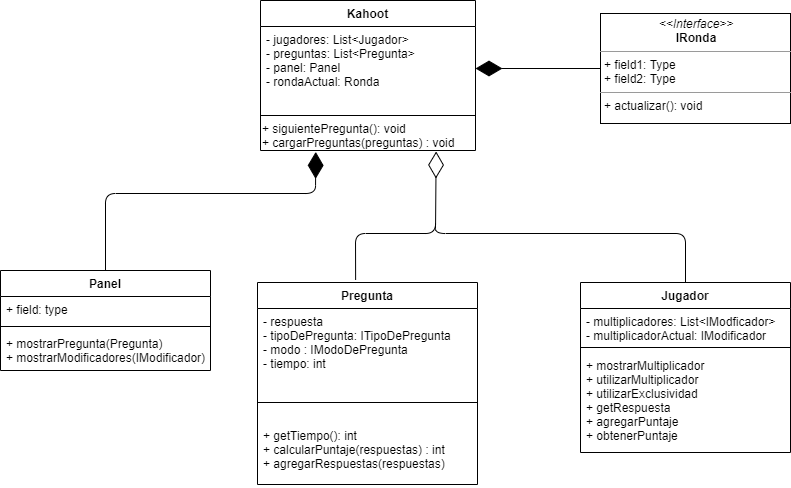
\includegraphics[width=0.8\textwidth]{diagramaGeneral.png}
\caption{\label{fig:class01}Diagrama del Kahoot.}
\end{figure}

\begin{figure}[H]
    \centering
    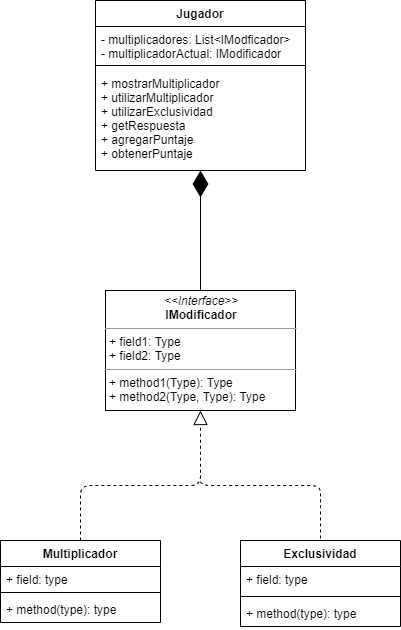
\includegraphics[width=0.8\textwidth]{diagramaJugador.png}
    \caption{\label{fig:class02}Diagrama del Jugador.}
\end{figure}

\begin{figure}[H]
    \centering
    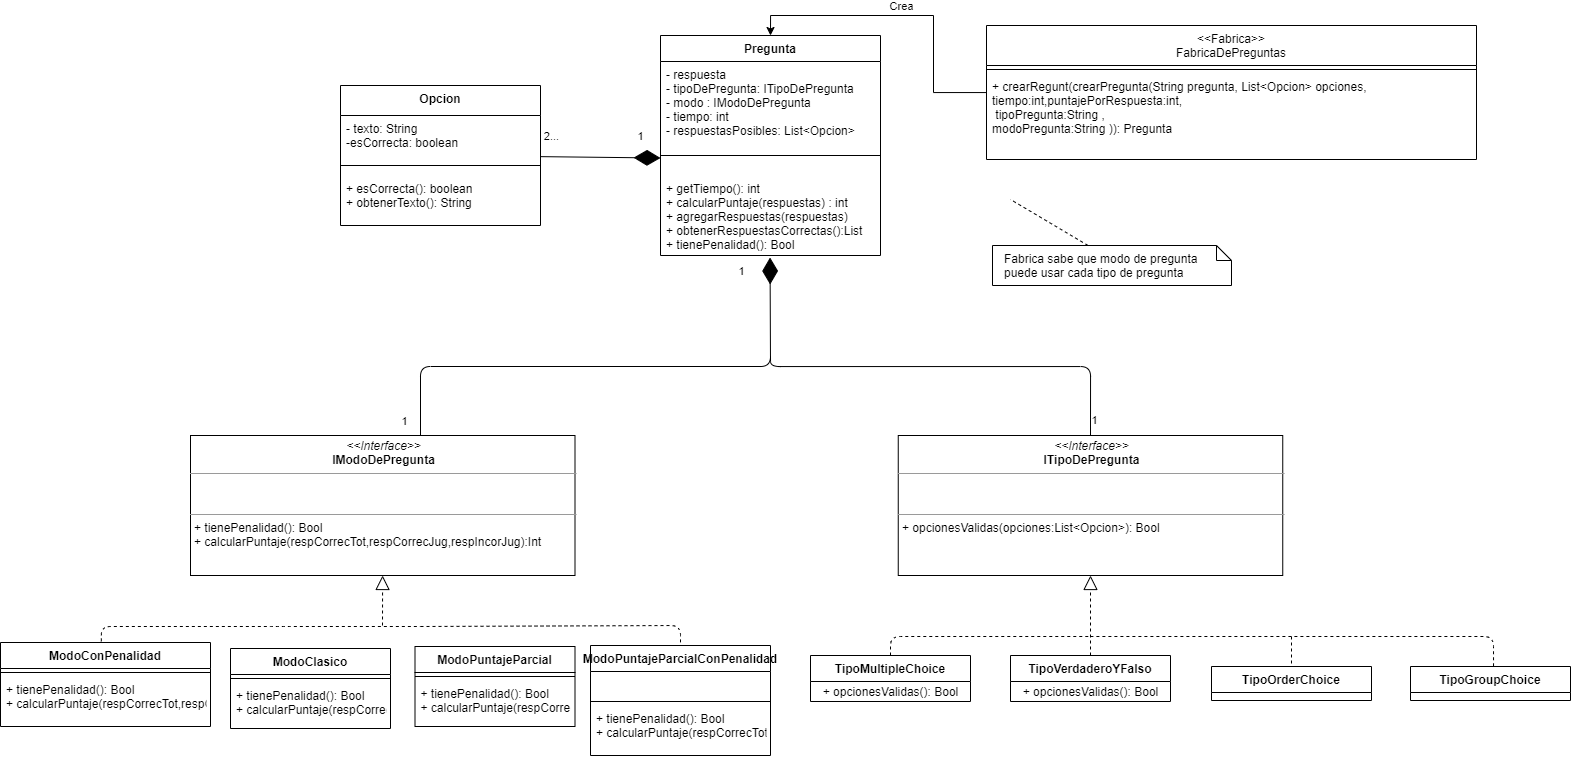
\includegraphics[width=0.8\textwidth]{diagramaPregunta.png}
    \caption{\label{fig:class03}Diagrama de Pregunta.}
\end{figure}

\begin{figure}[H]
    \centering
    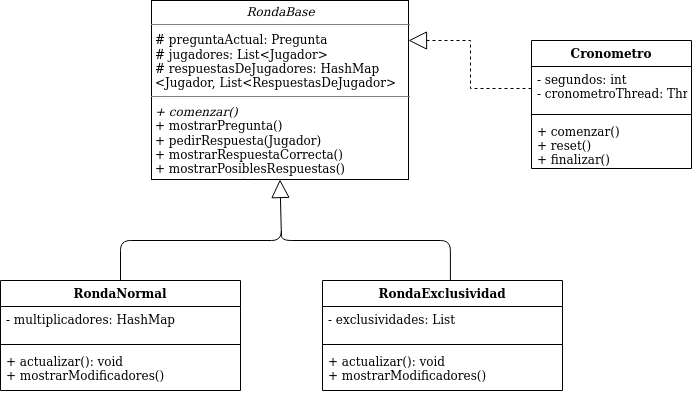
\includegraphics[width=0.8\textwidth]{diagramaRonda.png}
    \caption{\label{fig:class04}Diagrama de Ronda.}
\end{figure}


\section{Detalles de implementación}\label{sec:implementacion}
% Explicaciones sobre la implementación interna de algunas clases que consideren que puedan llegar a resultar interesantes.

\subsection{Inicializacion de preguntas}
Actualmente le proveemos dos formas distintas de cargar las preguntas al programa.

\begin{description}
{\bf Formato Propio}\newline
El archivo con el que inicializamos las preguntas contenia las lineas con el siguiente formato Modo/Tipo/Pregunta/Opciones/OpcionCorrecta .\newline
\newline

Siendo el contenido de cada campo el siguiente:\newline
\newline

Modo: String\newline
\indent- ConPuntajePenalidad\newline
\indent- Clasico\newline
\indent- Parcial\newline
\newline

Tipo: String\newline
\indent- MultipleChoice\newline
\indent- VerdaderoFalso\newline
\indent- OrderedChoice\newline
\indent- GroupChoice\newline
\newline

Pregunta: String\newline
\newline
Opciones: String,String,String\newline
\newline
OpcionCorrecta: String\newline
\newline

Ejemplo:\newline
\item
\begin{verbatim}
Clasico/MultipleChoice/¿Como se llama tu mascota?/Nestor,Chewbacca,Godzilla/Godzilla
\end{verbatim}
\newline

\end{description}

\begin{description}
{\bf Formato JSON}

\newline
\newline
El formato JSON mantiene la misma idea de formato propio, representando a los modos, las opciones y las preguntas como strings pero la diferencia principal es que estan separadas por categorias y que se utilizan los arrays que provee el formato JSON

\newline
\newline
Ejemplo de archivo MultiplChoice / VerdaderoYFalso 
\begin{verbatim}
{
  "MultipleChoice" :
      [{
        "modo": "ConPuntajeParcial",
        "texto" : "¿Quién gano gran hermano 2015?",
        "opciones" : ["Matías Schrank", "Francisco Delgado", "Vos"],
        "opcionesCorrectas": ["Francisco Delgado"],
      }]
}
\end{verbatim}
\newline
Ejemplo de archivo OrderedChoice / GroupChoice
\begin{verbatim}
{
"GroupChoice" :
      [{
        "modo": "Clasico",
        "texto" : "Separe entre caballos (Grupo 1) y flores (Grupo 2).",
        "opciones" : {"1": ["ANDALUZ", "APALUSA"], "2": ["NARCISOS"]}
      }]
}

{
  "OrderedChoice":
  [
    {
      "modo": "Clasico",
      "texto": "¿Cuál es el orden de nacimientos?",
      "opciones" : 
      {
        "1":["Jesus"],
        "2":["El Dieguito (maradona)"],
        "3":["Britney Spears"],
        "4":["Bad Luck Brian"]
      }
    }
  ]
}
\end{verbatim}
\end{description}

\subsection{Proin sodales leo dapibus sapien fermentum}
Quisque tempus, tortor et convallis interdum, ipsum leo tempus ipsum, in molestie tortor arcu sit amet tellus. Praesent fermentum hendrerit nulla. In maximus ornare maximus. Nullam consectetur placerat enim sit amet lacinia. Etiam pellentesque tellus consectetur hendrerit iaculis. Sed non laoreet felis.

\section{Excepciones}\label{sec:excepciones}
% Explicación de cada una de las excepciones creadas y con qué fin fueron creadas.

\begin{description}
\item[ExtensionInvalidaExcepcion] Esta excepcion fue creada con el fin de notificar al usuario que el archivo de preguntas que se dio tiene una extension erronea.
\item[NoQuedanUsosExcepcion] Esta excepcion fue creada con el fin de notificar al usuario que el Multiplicador que se utilizo no tenia usos disponibles y por ende la ejecucion no puede continuar.
\end{description}

\section{Diagramas de secuencia}\label{sec:diagramasdesecuencia}
% Mostrar las secuencias interesantes que hayan implementado. Pueden agregar texto para explicar si algo no queda claro.

\begin{figure}[H]
\centering
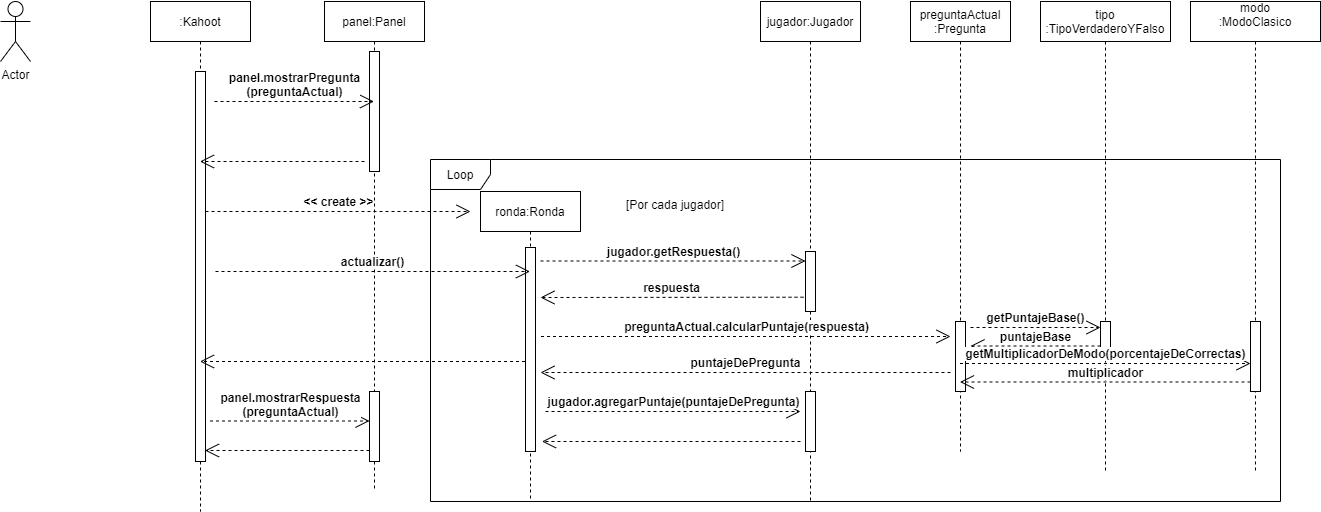
\includegraphics[width=0.8\textwidth]{diagramaDeSecuencia.png}
\caption{\label{fig:seq01}Se muestra el proceso de una ronda en el que un jugador responde una pregunta, se calcula el puntaje y se le agregan los puntos obtenidos.}
\end{figure}

\section{Diagrama de paquetes}\label{sec:diagramasdepaquetes}
\newline
En esta sección vamos a mostrar los paquetes del proyecto, así como sus dependencias, quién conoce a quién y con quién se comunican los jugadores.

\begin{figure}[H]
\centering
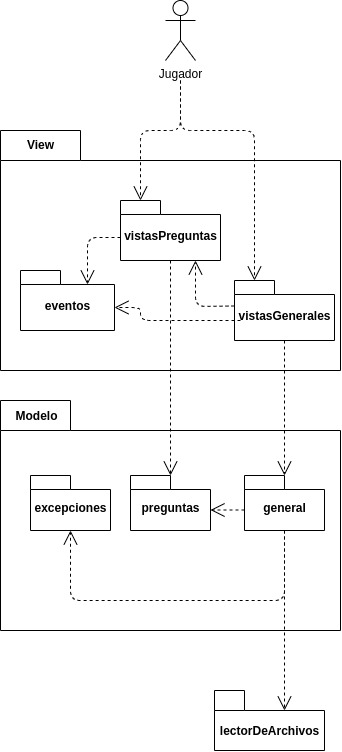
\includegraphics[width=0.8\textwidth]{DiagramaDePaquetes.jpg}
\caption{\label{fig:seq02}Podemos observar los distintos paquetes que se crearon en el proyecto.}
\end{figure}

\section{Diagramas de estado}\label{sec:diagramasdeestados}

En el primer diagrama se pueden ver los distintos estados que existen en la clase Exclusividad. Estos van a depender de la cantidad de usos disponibles que haya para el dado modificador de tipo exclusividad, siendo la cantidad inicial 2. En los primeros 2 estados, el comportamiento de la clase es el esperado y normal(aplica la exclusividad), pero una vez que pase por estos levantara la  excepcion "no tiene usos".
Tambien se puede notar que una vez que se utiliza la exclusividad, no se puede volver a un estado anterior por lo que solo hay un camino de transicion de estados.

\begin{figure}[H]
    \centering
    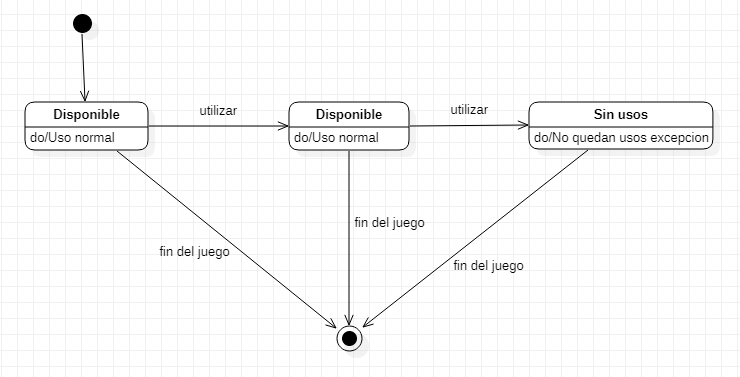
\includegraphics[width=0.8\textwidth]{DiagramaDeEstadoExclusividad.png}
    \caption{\label{fig:class03}Diagrama de exclusividad.}
\end{figure}

El segundo diagrama trata de una clase similar a la mencionada anteriormente, con la excepcion de que solo se tiene un uso al inicializarse. Ademas, al ingresar al estado "Disponible" que vendria a ser cuando se inicialice el objeto para un dado jugador, se creara un factor dependiendo del parametro.

\begin{figure}[H]
    \centering
    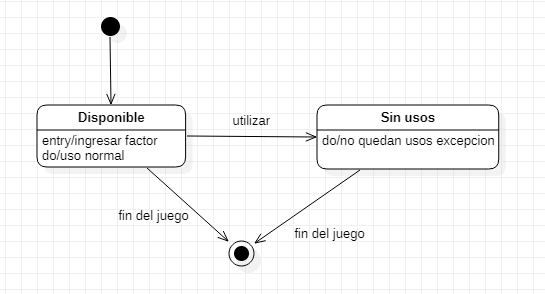
\includegraphics[width=0.8\textwidth]{DiagramaDeEstadoMultiplicador.png}
    \caption{\label{fig:class04}Diagrama de multiplicador.}
\end{figure}

En el ultimo diagrama se pueden  ver las distintas transiciones de estado internas que tiene el cronometro. Se puede observar que si se usa el metodo de esperar 1 segundo, se vuelve a un estado anterior. Los distintos estados van a estar creados por los pulsos de reloj.

\begin{figure}[H]
    \centering
    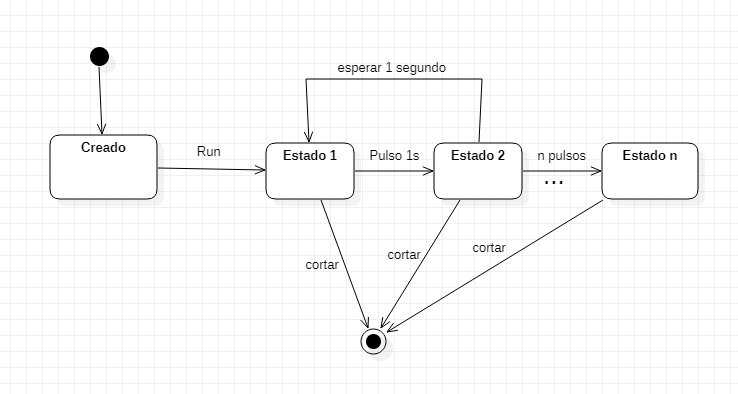
\includegraphics[width=0.8\textwidth]{DiagramaDeEstadoCronometro.png}
    \caption{\label{fig:class05}Diagrama de cronometro.}
\end{figure}


\end{document}
